\documentclass[12pt,a4paper]{article}
\usepackage[utf8]{inputenc}
\usepackage[french]{babel}
\usepackage[T1]{fontenc}
\usepackage{amsmath}
\usepackage{amsfonts}
\usepackage{amssymb}
\usepackage{graphicx}
\usepackage[left=2cm,right=2cm,top=2cm,bottom=2cm]{geometry}
\title{DOCUMENTATION DOCKER \textbf{Docker}}
\begin{document}
\maketitle
\section{Plan de cours}

\begin{tabular}{|c|p{12cm}|}
\hline 
Séance & chapitre \\ 
\hline 
1 & \begin{itemize}
\item[•] Généralité.
\item[•] Installer docker.
\item[•] Lancer notre première container.
\end{itemize} \\ 
\hline 
2 & \begin{itemize}
\item[•] Dockerfile : Créer une image.
\item[•] Fonctionnement du cache.
\end{itemize} \\ 
\hline 
3 & \begin{itemize}
\item[•] Comprendre les Layers / Couches.
\item[•] Les Réseaux.
\item[•] Docker Compose.
\item[•] ENTRYPOINT VS CMD.
\end{itemize} \\ 
\hline 
4 & \begin{itemize}
\item[•] Sécuriser le user namespace.
\item[•] Dokerfile multi-stage.
\item[•] Les images: TAGS, PULL ET PUSH.
\item[•] L'API Docker.
\end{itemize} \\ 
\hline 
5 & \begin{itemize}
\item[•] Développent des modules pour \textbf{PORTE-IFNTI}.
\end{itemize} \\ 
\hline 
\end{tabular} 

\section{Généralités}
Dans cette première partie, nous allons découvrir les \textbf{conteneurs} ainsi qu'avec 
Docker. Mais avant cela, nous allons revenir sur quelque notions importantes :
\begin{itemize}
\item[•] comprendre la notion de \textbf{machine virtuelle};
\item[•] comprendre la notion de \textbf{conteneur};
\item[•] \textbf{pourquoi} utiliser les conteneurs ?
\end{itemize} 
\subsection{Machine virtuelle (VM)}
Utiliser une machine virtuelle c'est faire de la \textbf{virtualisation lourde}. Pourquoi car
nous recréons un système complet (avec ses propres ressource) dans notre système.

\textbf{L'isolation avec le système hôte est donc totale}; cependant cela nous apporte 
plusieurs contraintes et avantages.
\begin{itemize}
\item[] Contraint.
\begin{itemize}
\item[•] Une machine virtuelle prend du \textbf{temps} à démarrer;
\item[•] Une machine virtuelle \textbf{réserve les ressources (CPU/RAM)} sur le système 
hôte.
\end{itemize}
\item[] Avantages.
\begin{itemize}
\item[•] Une machine virtuelle est totalement \textbf{isolée} du système hôte;
\item[•] Les ressource attribuées à une machine virtuelle lui sont totalement \textbf{réservées}.
\item[•] Vous pouvez installer \textbf{différents OS} (Linux, Windows, etc.).
\end{itemize}

\begin{figure}[!t]
\centering
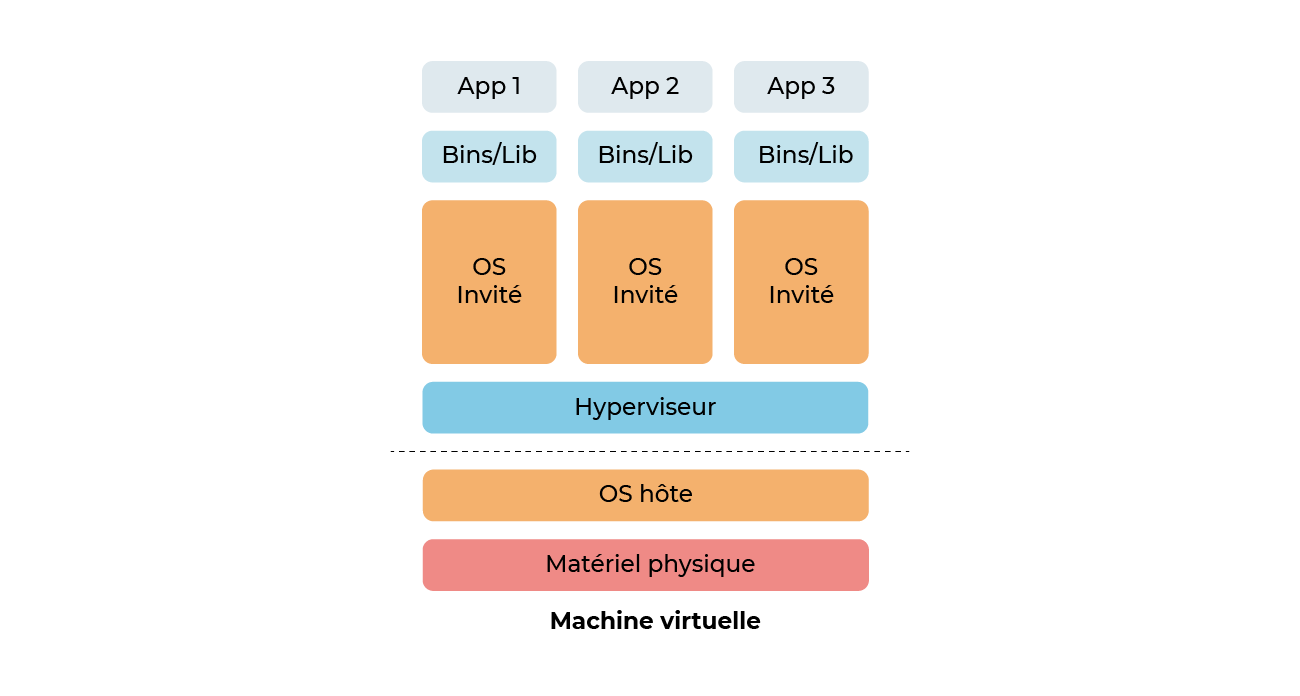
\includegraphics[scale=0.3]{img/vm.png}
\caption{Fonctionnement d'une machine virtuelle}
\label{Tux}
\end{figure}

Mais il arrive souvent que l'application qu'elle fait tourner ne consomme pas l'ensemble 
des ressources disponibles sur la machine virtuelle. Alors est né un nouveau système de 
virtualisation plus léger : les \textbf{conteneurs}.
\end{itemize}
\subsection{Conteneur}
Un conteneur Linux est un \textbf{processus} ou un ensemble de processus isolés du reste du
système, tout en étant \textbf{légers}.\\
Le conteneur permet de faire de la \textbf{virtualisation légère}, c'est à dire qu'il ne virtualise pas les ressources, il ne crée qu'une \textbf{isolation des processus}. Le conteneur partage donc les ressources avec le système hôte.\\

\textbf{Attention}, les conteneurs existent depuis plus longtemps que \textbf{Docker}.
\textbf{OpenVZ} ou \textbf{LXC} sont des technologies de conteneur qui existent depuis de
nombreuses années.

Les conteneurs, au sens d'OpenVZ et LXC, apportent une \textbf{isolation importante des processus systèmes} ; cependant, les ressources CPU, RAM et disque sont totalement
partagées avec l'ensemble du système. Les conteneurs partagent entre eux le kernel Linux;
ainsi, il n'est pas possible de faire fonctionner un système Windows ou BSD dans celui-ci.

\begin{figure}[!t]
\centering
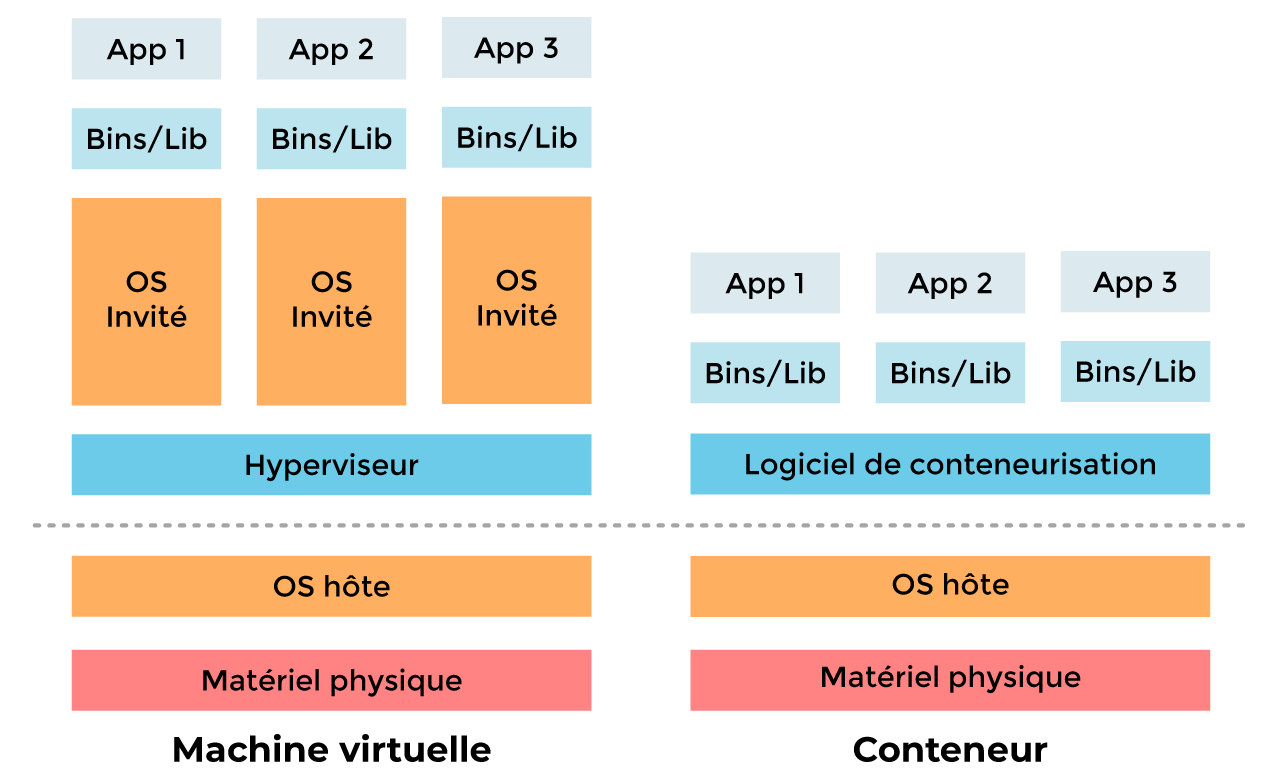
\includegraphics[scale=0.3]{img/container_vs_vm.png}
\caption{Fonctionnement d'une machine virtuelle}
\label{Tux}
\end{figure}

Maintenant voyons quelque exemple des conteneurs.
\begin{itemize}
\item \textbf{Ne réservez que les ressources nécessaires}
Une autre différence importante avec les machines virtuelles est qu'un conteneur \textbf{ne réserve pas} la quantité de CPU, RAM et disque attribuée auprès du système hôte. Ainsi, nous pouvons allouer 16 Go de RAM à notre conteneur, mais si celui-ci n'utilise que 2 Go, le reste ne sera pas verrouillé.
\item \textbf{ Démarrez rapidement vos conteneurs}
Les conteneurs n'ayant pas besoin d'une virtualisation des ressources mais seulement d'une isolation, ils peuvent \textbf{démarrer beaucoup plus rapidement} et plus fréquemment qu'une machine virtuelle sur nos serveurs hôtes, et ainsi réduire encore un peu les frais de l'infrastructure.
\item \textbf{Donnez plus d'autonomie à vos développeurs}
En dehors de la question pécuniaire, il y a aussi la possibilité de faire tourner des conteneurs sur le poste des développeurs, et ainsi de réduire les différences entre la "sainte" production, et l'environnement local sur le poste des développeurs.
\end{itemize}

\subsection{Pourquoi utiliser des conteneurs ?}
Les conteneurs permettent de \textbf{réduire les coûts}, d'augmenter la \textbf{densité de l'infrastructure}, tout en améliorant le cycle de déploiement.

Grace à leur capacité de démarrer plus rapidement, les conteneurs sont souvent utilisés en 
production pour ajouter des ressources disponibles, et ainsi répondre à des besoins de mise
à l'échelle ou de scalabilité. Mais ils répondent aussi à des besoins de préproduction;
en étant légers et rapides au démarrage, il permettent de créer des environnements dynamique et ainsi de répondre à des besoins métier.

\section{Docker}
\subsection{Une petite histoire}
Docker a été créé pour les besoins d'une société de Platform as a Service (PaaS) appelée \textbf{DotCloud}. Finalement, en mars 2013, l'entreprise a créé une nouvelle structure nommée \textbf{Docker Inc} et a placé en open source son produit \textbf{Docker}.

\subsection{Objectifs}
Docker apporte une notion importante dans le monde du conteneur. Dans la vision Docker, un conteneur ne doit faire tourner qu'\textbf{un seul processus}. Ainsi, dans le cas d'une stack LAMP (Linux, Apache, MySQL, PHP), nous devons créer \textbf{3 conteneurs} différents, un pour Apache, un pour MySQL et un dernier pour PHP. Alors que dans un conteneur LXC ou OpenVZ, nous aurions fait tourner l'ensemble des 3 services dans un seul et unique conteneur.

\subsection{Pourquoi utiliser Docker ?}
Docker répond à une problématique forte dans le monde du développement.
Prenons un exemple : vous avez développé votre projet de Twitter Lite en local. Tout fonctionne bien, mais au moment de mettre en production, vous vous rendez compte que vous ne savez pas comment \textbf{déployer votre projet}. Un autre exemple : vous êtes dans une équipe de 10 personnes et chacun utilise un OS différent (Ubuntu, macOS, Windows, CentOS, etc.). Comment faire pour avoir \textbf{un environnement unifié et fonctionnel} chez l'ensemble des développeurs ?

Docker répond à ces problématiques en créant des conteneurs. Grâce à Docker, vous n'aurez plus de problème de différence d'environnement, et votre code marchera partout !

\subsection{Installer Docker}
Docker Inc distribue 3 versions de Docker différentes :
\begin{itemize}
\item[•] Docker Community Edition (Linux seulement) ;
\item[•] Docker Desktop (Mac ou Windows) ;
\item[•] Docker Enterprise (Linux seulement).
\end{itemize}
Docker Desktop et Docker Community Edition (CE) sont deux versions de Docker gratuites. Avec les deux solutions, vous aurez un Docker fonctionnel sur votre ordinateur.

Si vous êtes sous Windows ou macOS, utilisez Docker Desktop qui va créer pour vous l'ensemble des services nécessaires au bon fonctionnement de Docker.

Si vous êtes sous Linux, prenez la version Community Edition (CE) ; vous utiliserez aussi cette version pour vos serveurs.

La version Docker Enterprise ne ressemble pas du tout aux versions Desktop et CE. Celle-ci répond à des besoins plus poussés des entreprises, et propose une interface de gestion d'infrastructures sous Docker. Cette version est soumise à une licence fournie par Docker Inc.

\textbf{NB:} Pour installer docker sur Mac ou Windows rendez vous ici.
Dans le cas de Linux, vous devez utiliser les commandes suivante.
\begin{verbatim}
sudo aptget install docker.io
\end{verbatim}

Après ou avant l'installation de docker il est conseiller de créer votre compte au
niveau 

\section{Lancer notre premier conteneur}
Dans cette partie, je vous propose de \textbf{prendre en main Docker}. Nous allons 
commencer par découvrir l'\textbf{interface en ligne de commande}, qui nous permet
de discuter avec le \textbf{daemon Docker} installé précédemment. D'ici la fin de cette partie, vous serez capable de \textbf{lancer et gérer vos conteneurs}. Mais commençons dans ce chapitre par comprendre ce qu'est le \textbf{Docker Hub}, puis nous lancerons notre \textbf{premier conteneur}.

\subsection{Le Docker Hub}
Avant de démarrer votre premier conteneur Docker, rappelez-vous quand vous avez créé votre compte sur le Docker Hub pour télécharger votre version de Docker. Celui-ci est aussi 
\textbf{la registry officielle de Docker}.\\

Une \textbf{registry} est un logiciel qui permet de partager des images à d'autres personnes. C’est un composant majeur dans l’écosystème Docker, car il permet :

\begin{itemize}
\item à des développeurs de distribuer des images prêtes à l’emploi et de les versionner avec un système de tags ;
\item à des outils d’intégration en continu de jouer une suite de tests, sans avoir besoin d’autre chose que de Docker ;
\item à des systèmes automatisés de déployer ces applications sur vos environnements de développement et de production.
\end{itemize}

\subsection{Démarrez votre premier conteneur Docker}
Pour démarrer votre premier conteneur, vous devez utiliser la commande :
\begin{verbatim}
docker run hello-world
\end{verbatim}
\begin{center}
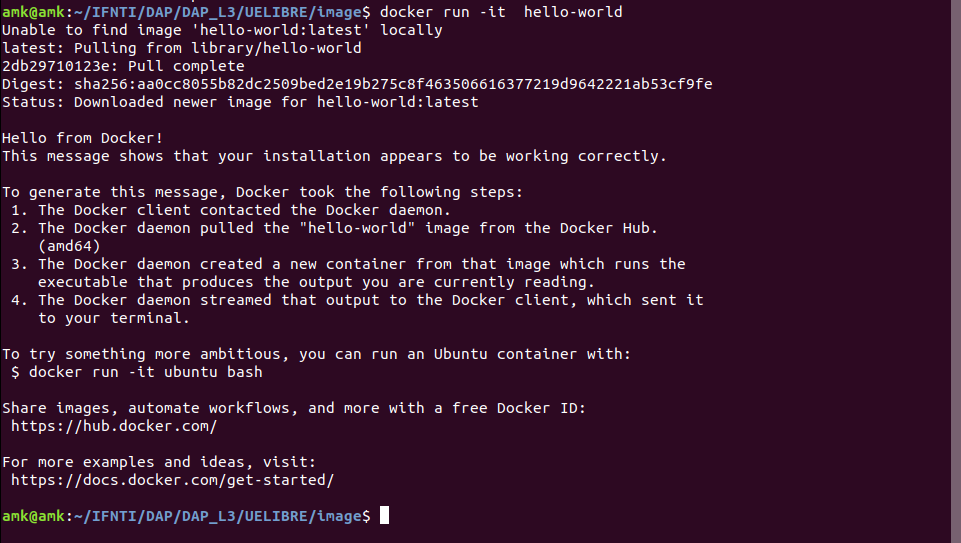
\includegraphics[scale=0.3]{img/p_conteneur.png}
\end{center}
Quand vous utilisez cette commande, le \textbf{daemon Docker} va chercher si l'image \textit{hello-world} est \textbf{disponible en local}. Dans le cas contraire, il va la \textbf{récupérer sur la registry Docker officielle.}

Dans notre cas, le conteneur a démarré, puis affiché du contenu, et il a fini par s'arrêter. Si vous souhaitez \textbf{que votre conteneur reste allumé jusqu’à l'arrêt du service qu'il contient}, vous devez ajouter l’argument \textit{- -detach (-d)} . Celui-ci permet de ne pas rester attaché au conteneur, et donc de pouvoir lancer plusieurs conteneurs. Nous allons voir dans la section suivante comment utiliser l’argument -d.

\subsection{Démarrez un serveur Nginx avec un conteneur Docker}
vous savez lancer un conteneur, et vous avez compris les actions effectuées par le daemon Docker lors de l'utilisation de la commande docker run.

Maintenant, nous allons aller plus loin avec celui-ci. Nous allons lancer un conteneur qui démarre un serveur Nginx en utilisant deux options (\textbf{-d} et \textbf{-p}) :
\begin{verbatim}
docker run -d -p 8080:80 nginx 
\end{verbatim}  .
Dans cette commande, nous avons utilisé deux options :
\begin{itemize}
\item -d pour détacher le conteneur du processus principal de la console. Il vous permet de continuer à utiliser la console pendant que votre conteneur tourne sur un autre processus ;
\item -p pour définir l'utilisation de ports. Dans notre cas, nous lui avons demandé de transférer le trafic du port 8080 vers le port 80 du conteneur.
\end{itemize}
    Ainsi, en vous rendant sur l'adresse  http://127.0.0.1:8080, vous aurez la page par défaut de Nginx.\\
Vous pourriez aussi avoir besoin de "rentrer" dans votre conteneur Docker pour pouvoir y effectuer des actions. Pour cela, vous devez utiliser la commande 
\textbf{docker exec -ti ID\_RETOURNÉ\_LORS\_DU\_DOCKER\_RUN bash}  . Dans cette commande, l'argument \textit{-ti} permet d'avoir un shell bash pleinement opérationnel. Une fois que vous êtes dans votre conteneur, vous pouvez vous rendre, via la commande \textbf{cd /usr/share/nginx/html}  , dans le répertoire où se trouve le fichier index.html  , pour modifier son contenu et voir le résultat en direct à l'adresse http://127.0.0.1:8080.

\subsection{Récupérez une image depuis le docker Hub}
Vous pouvez aussi avoir besoin de récupérer des images sur le Docker Hub sans pour autant lancer de conteneur. Pour cela, vous avez besoin de lancer la commande suivante :

\begin{verbatim}
 docker pull hello-world

Using default tag: latest

latest: Pulling from library/hello-world

Digest: sha256:2557e3c07ed1e38f26e389462d03ed943586f744621577a99efb77324b0fe535

Status: Image is up to date for hello-world:latest
\end{verbatim}

En lançant cette commande, vous téléchargez une image directement depuis le Docker Hub, et vous la stockez en local sur votre ordinateur.

\textbf{NB : } Généralement le pull d'une image peut prendre, beaucoup de seconde voir minute.

\subsection{Quelles que commandes}
\begin{itemize}
\item[•] \textbf{docker images} ou \textbf{docker image ls} : Affiche la liste de toute les
images.
\begin{center}
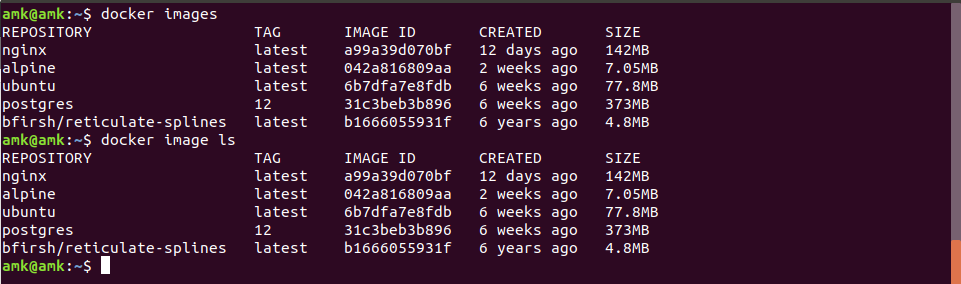
\includegraphics[scale=0.5]{img/docker_images.png}
\end{center}
On peut facilement repérer les métadonnées suivantes :
\begin{verbatim}
REPOSITORY                  TAG       IMAGE ID       CREATED       SIZE
\end{verbatim}
\begin{itemize}
\item \textbf{REPOSITORY} désigne souvent le nom de l'image.
\item \textbf{TAG} sa version.
\item \textbf{IMAGE ID} son identifiant (unique).
\item \textbf{CREATED} l'heur à la quelle elle à été créer et enfin
\item \textbf{SIZE} L'espace mémoire quelle occupe.
\end{itemize}
\item[•] \textbf{docker ps} ou \textbf{docker container ls} : Affiche la liste de tous les
conteneurs dans l'état \textbf{RUNING}. pour afficher tous les conteneurs vous allez 
devoir spécifier l'option \textbf{-a} pour \textit{all}.
\item[•] \textbf{docker stop ID\_RETOURNÉ\_LORS\_DU\_DOCKER\_RUN} permet d'arrêter un conteneur.
\item[•] \textbf{docker rm ID\_RETOURNÉ\_LORS\_DU\_DOCKER\_RUN} ou \textbf{docker rm NOM\_CONTENEURE} permet de supprimer un conteneur.\\
\textbf{NB : } Cela ne fonctionnera si et seulement si le conteneur est stoppé. Pour 
contourner ce problème vous pouvez utiliser l'option -f (pour \textit{force}) comme ceci
\textbf{docker rm -f ID\_RETOURNÉ\_LORS\_DU\_DOCKER\_RUN} 
\item[•] \textbf{docker image rm IMAGE\_ID} ou \textbf{docker rmi IMAGE\_ID} permet 
de supprimez une image. Vous pouvez aussi utiliser ici l'option -f.
\item[•] \textbf{docker inspect ID\_RETOURNÉ\_LORS\_DU\_DOCKER\_RUN} pour avoir
des détails plus détaillé sur le conteneur.
\end{itemize}

\subsection{Comment nettoyer son système docker}
Après avoir fait de nombreux tests sur votre ordinateur, vous pouvez avoir besoin de faire un peu de ménage. Pour cela, vous pouvez supprimer l'ensemble des ressources manuelles dans Docker.\\
Ou vous pouvez laisser faire Docker pour qu'il fasse lui-même le ménage. Voici la commande que vous devez utiliser pour faire le ménage :  \textbf{docker system prune}.\\
\begin{verbatim}
 docker system prune
WARNING! This will remove:
- all stopped containers
- all networks not used by at least one container
- all dangling images
- all dangling build cache
Are you sure you want to continue? [y/N] y
Deleted Containers:
941b8955b4fd8988fefe2aa91c7eb501f2d4f8c56bf4718fea8ed50904104745
a96e73c623fb6530ab41db6a82aca7017d54a99590f0b45eb6bf934ef8e4d3ed

Deleted Images:
deleted: sha256:797a90d1aff81492851a11445989155ace5f87a05379a0fd7342da4c4516663e
deleted: sha256:c5c8911bd17751bd631ad7ed00203ba2dcb79a64316e14ea95a9edeb735ca3ea

Total reclaimed space: 21.08MB
\end{verbatim}
Celle-ci va supprimer les données suivantes :
\begin{itemize}
\item[•] l'ensemble des conteneurs Docker qui ne sont pas en status running ;
\item[•] l'ensemble des réseaux créés par Docker qui ne sont pas utilisés par au moins un conteneur ;
\item[•] l'ensemble des images Docker non utilisées ;
\item[•] l'ensemble des caches utilisés pour la création d'images Docker.
\end{itemize}

\section{Les Volumes}
Lorsque vous créer un conteneur, par défaut ses données ne sont pas
persistant. C'est à dire que si vous supprimé un conteneur ses
données disparaîtrons aussi. Pour éviter que cela ne se produise
docker à mis en place la notion de volume.\\
\textbf{Docker volume} est un \textbf{mécanisme de fichiers géré
par Docker permettant de sauvegardé des données générées lors de 
l'exécution d'un conteneur}. Il permet également de monter les données dont le conteneur a besoin à l'intérieur de ce dernier lors
de son lancement.\\
Mais avant de voir \textbf{Docker volume} nous allons voir les
volume persistant.

\subsection{Les volumes persistant}
Vous vous souvenez du serveur nginx que nous avions créer ? si 
vous l'avez déjà supprimé, je vous pris de le recréer. Voici
la commande si vous l'avez oublié
\begin{verbatim}
docker run -d --name seveur -p 8080:80 nginx
\end{verbatim}
Une fois créer entrer dans le conteneur en utilisant la commande suivante :
\begin{verbatim}
docker exec -it serveur
\end{verbatim}
Rendez-vous ensuite dans le fichier index.html et modifier le à votre guise. Mais souvenez vous il n'y pas de vim ou de nano par
\begin{center}
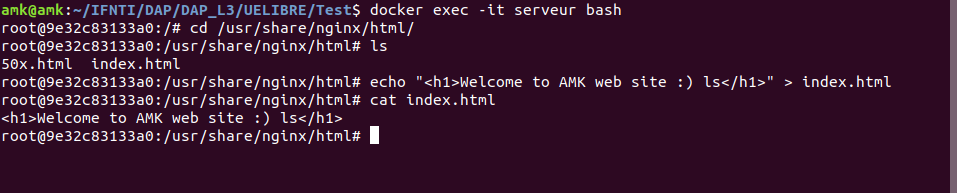
\includegraphics[scale=0.3]{img/volume_persistant_1.png}
\end{center}
Voici le résultat.
\begin{center}
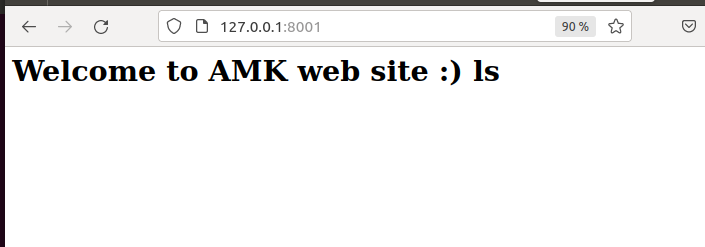
\includegraphics[scale=0.3]{img/volume_persistant.png}
\end{center}
Maintenant supprimé votre conteneur et recréer le.
\begin{verbatim}
docker rm -f serveur
docker run -d --name serveur -p 8080:80 nginx
\end{verbatim}
Que se passe t-il ?
Vos modification n'ont pas été pris en compte et vous voyez la
page par défaut de nginx ! 
Pour régler ce problème nous allons utiliser un volume. créer un 
répertoire nommé \textbf{public\_html}. Créez s'y le fichier
\textbf{index.html}(mettez y ce que vous voulez).
Comme la redirection de port, nous allons 
faire le mappage de répertoire en disant que le répertoire 
\textbf{/urs/share/nginx/html} doit correspondre au répertoire
\textbf{public\_html}. Vous comprenez donc pourquoi nous devons 
créer nous même le fichier \textbf{index.html}. Créez maintenant
notre conteneur.
\begin{verbatim}
docker run -d --name serveur -p 8001:80 -v /home/amk/IFNTI/DAP/DAP_L3/UELIBRE/Test/test/public_html/:/usr/share/nginx/html/ nginx 
\end{verbatim}
\begin{center}
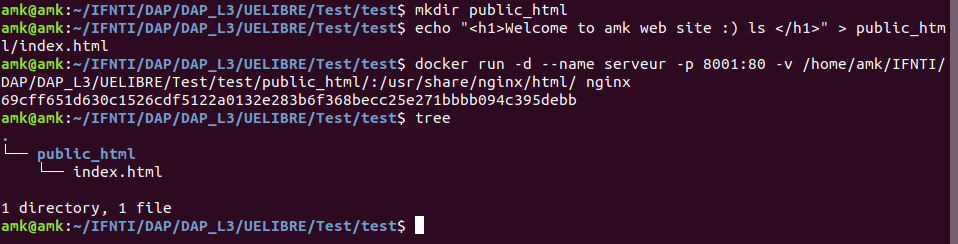
\includegraphics[scale=0.3]{img/volume_mount.png}
\end{center}
Supprimer votre conteneur et recréer le que se passe t'il ?
Vos données sont devenue persistant ! C'est cool n'est pas.
\begin{center}
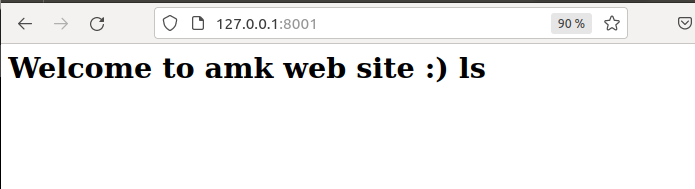
\includegraphics[scale=0.3]{img/test_volume.png}
\end{center}
Dans la suit nous allons voir docker volume.

\subsection{Docker volume}
Docker volume nous permet de créer des volumes à volonté. Par
défaut les volumes que nous créer on leurs point de montage au
niveau de la machine hôte dans le répertoire \textbf{/var/lib/
docker/volumes/}.\\
Pour voir tous ce qu'on peut faire avec docker volume (et cela vaut
pour toute les commande) vous n'avez
qu'a taper \textbf{docker volume} dans votre terminal vous verrez
ça.
\begin{verbatim}
amk@amk:~/IFNTI/DAP/DAP_L3/UELIBRE/Test/test$ docker volume 

Usage:  docker volume COMMAND

Manage volumes

Commands:
  create      Create a volume
  inspect     Display detailed information on one or more volumes
  ls          List volumes
  prune       Remove all unused local volumes
  rm          Remove one or more volumes

Run 'docker volume COMMAND --help' for more information on a command.
amk@amk:~/IFNTI/DAP/DAP_L3/UELIBRE/Test/test$ 

\end{verbatim}
Nous allons créer un volume nommé monvolume voici la commande.
\begin{verbatim}
amk@amk:~/IFNTI/DAP/DAP_L3/UELIBRE/Test/test$ docker volume create monvolume
monvolume
amk@amk:~/IFNTI/DAP/DAP_L3/UELIBRE/Test/test$ 
\end{verbatim}
Pour avoir plus de détails sur un volume vous utiliser la commande
inspect comme ceci.
\begin{verbatim}
amk@amk:~/IFNTI/DAP/DAP_L3/UELIBRE/Test/test$ docker volume inspect monvolume 
[
    {
        "CreatedAt": "2023-01-25T10:07:02Z",
        "Driver": "local",
        "Labels": {},
        "Mountpoint": "/var/lib/docker/volumes/monvolume/_data",
        "Name": "monvolume",
        "Options": {},
        "Scope": "local"
    }
]
amk@amk:~/IFNTI/DAP/DAP_L3/UELIBRE/Test/test$ 
\end{verbatim}
Maintenant nous allons utiliser notre volume sur un conteneur en
utilisant l'option \textbf{--mount}
\begin{verbatim}
docker run -d --name web -p 8001:80 --mount source=monvolume,target=/usr/share/nginx/html nginx
\end{verbatim}
Voici le résultat:
\begin{center}
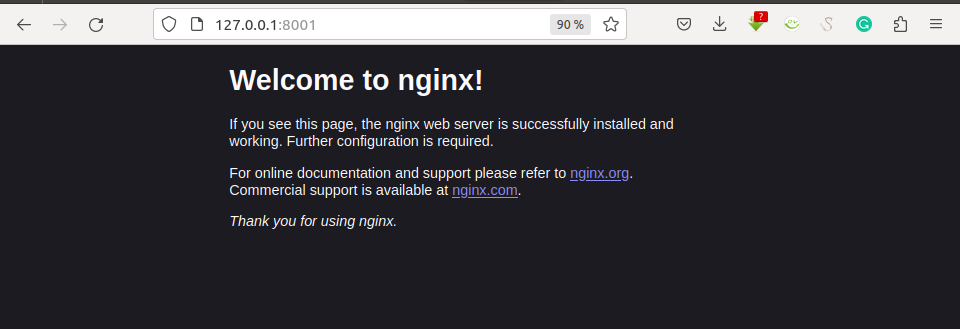
\includegraphics[scale=0.3]{img/docker_volume_init.png}
\end{center}
Vous pouvez modifier le contenue du fichier index.php comme ceci:
\begin{verbatim}
sudo vim /var/lib/docker/volumes/monvolume/_data/index.html
\end{verbatim}
Voici le résultat:
\begin{center}
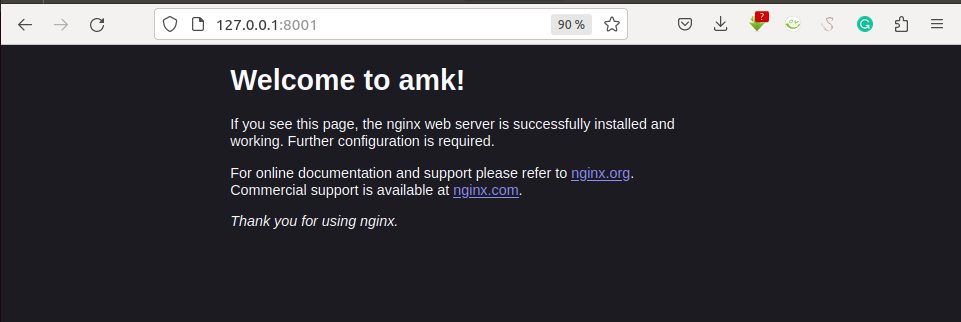
\includegraphics[scale=0.3]{img/docker_volume_n.png}
\end{center}
Maintenant que vous êtes maître amusé vous avec la commande
\textbf{docker volume}.

\section{Dockerfile : Créer une image.}
Vous savez maintenant utiliser l'interface de commande de Docker et récupérer des images depuis le Docker Hub. Mais comment créer votre propre image ?\\
Dans cette partie, nous allons créer ensemble une image Docker, dans laquelle nous allons installer nginx.\\
Pour cela, nous allons créer un fichier nommé \textbf{"Dockerfile"} (fichier de configuration). Dans ce fichier Dockerfile, vous allez trouver l'ensemble de la recette décrivant l'image Docker dont vous avez besoin pour votre projet.\\
Intérêts de \textbf{Dockerfile}.
\textit{À titre de comparaison, vous pouvez voir le Dockerfile comme l'équivalent d'un fichier package.json en Node.js, ou composer.json en PHP. } \\
Chaque instruction que nous allons donner dans notre Dockerfile va créer une nouvelle layer correspondant à chaque étape de la construction de l'image.
Notre est de limiter le nombre e layers, pour que image soit la plus légère et performante possible.

Voici quelles que closes d'un \textbf{Dockerfile}:
\begin{itemize}
\item[•] \textbf{RUN} : lancement de commande (apt...).
\item[•] \textbf{ENV} : variable d'environnement.
\item[•] \textbf{EXPOSE} : exposition de port.
\item[•] \textbf{VOLUME} : définition de volumes
\item[•] \textbf{COPY} : cp entre host et conteneur
\item[•] \textbf{ENTRYPOINT} : processus maître.
\item[•] \textbf{...} : ...
\end{itemize}

Voici le contenue de notre Dockerfile.

\begin{verbatim}
FROM nginx:latest
WORKDIR /usr/share/nginx/html/
RUN rm index.html
COPY . .
\end{verbatim}

Dans cette image on :
\begin{itemize}
\item part de la dernière version du serveur nginx,
\item définit le répertoire de travail,
\item supprime le fichier index.html
\item copie de notre fichier index.html.
\end{itemize} 

\textbf{NB}: \\
Il est capitale de nommé votre fichier \textbf{"Dockerfile"} tel quel.
Il est très important de toujours \textbf{partir d'une base} (FROM ...).
un fichier Dockerfile ne peut qu'avoir qu'une base.

Maintenant que vous savez pourquoi et comment créer un dockerfile il nous reste plus
qu'a l'exécuté. Pour lancer une image on utilise la commende suivante.

\textbf{docker build -t site\_html:v1.0 .}

Cette commande signifie que nous souhaitons créer une image dont le nom vaut \textit{site\_html}
et la version \textit{v1.0} en se servant du Dockerfile se trouvant dans notre répertoire 
courant (si vous ne spécifiez pas de version elle sera à latest pour dernière version).
si vous faite \textit{docker images} vous pouvez comme moi voir votre image .\\
::::::img\\
On peut aussi faire \textit{docker history site\_html:v1.0} pour voir en détails les étapes de 
la création de notre image.\\

On peut donc créer un conteneur à partir de notre image en utilisant la commande suivante:
\textbf{docker run -tid --name website site\_html:v1.0}

\section{Les Layers}
Les layers ou couches en français intervienne dans la création d'une image et d'un conteneur. Avec docker on peut distinguer deux types de couches :
\begin{itemize}
\item ceux en lecture seul (images).
\item et ceux en lecture-écriture (conteneurs).
\end{itemize} 
les images comme les conteneurs peuvent se partager au moins une couche.
:::::Expérience des couches xavki +
:::::Expérience de couche partagé.

\subsection{Le cache docker}
But du cache : 
\begin{itemize}
\item construire plus vite les images
\item démarrer plus vite les conteneurs
\item stocker des images légères
\item partage de couche/cache
\end{itemize}
Démonstration : \\
\subsubsection{Lancer deux fois de suite une image (using cache)}
Ici nous allons essayer de lancer deux fois de suite une même image. Voici 
le contenue su docker file contenue dans cette image.
\begin{verbatim}
FROM alpine:latest

LABEL maintener="amk"

RUN apk add vim
\end{verbatim}
lorsqu'on lance pour la première fois cette image avec la commande :
\begin{verbatim}
docker build -t test_vim .
\end{verbatim}
On peut remarqué qu'il n'a pas utilisation du cache.
\begin{center}
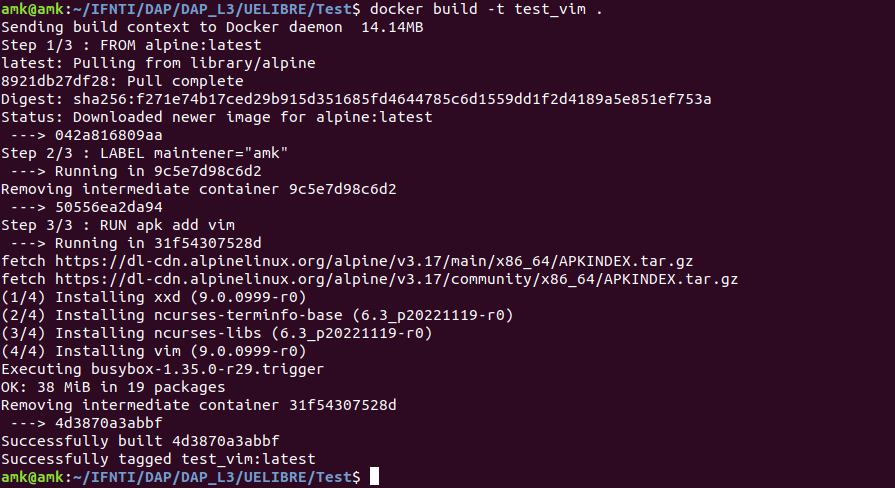
\includegraphics[scale=0.3]{img/test_vim.png}
\end{center}
Par contre si on relance une deuxième fois l'image là il y-a utilisation du cache.
\begin{center}
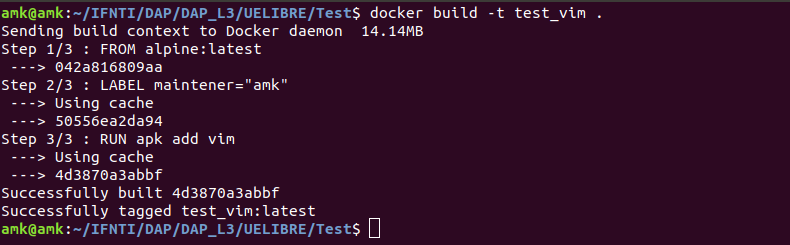
\includegraphics[scale=0.3]{img/test_vim_cache.png}
\end{center}
L'utilisation du cache se fait même si on change le nom de l'image comme ceci :
\begin{verbatim}
docker build -t test_vim2
\end{verbatim}
\begin{center}
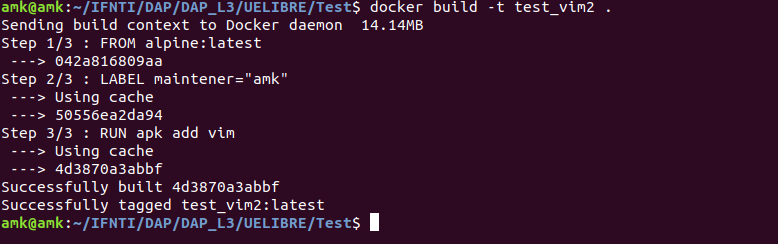
\includegraphics[scale=0.3]{img/test_vim3.png}
\end{center}
\textbf{Conclusion } : Une couche n'est télécharger que si elle n'existe pas.
\subsubsection{Ne pas cacher (--no-cache)}
On peut vouloir ne pas utiliser le cache lors du build d'une image. Dans ce cas notre image
sera comme ceci.
\begin{verbatim}
FROM alpine:latest

LABEL maintener="amk"

RUN apk add --no-cache vim
\end{verbatim}
\begin{center}
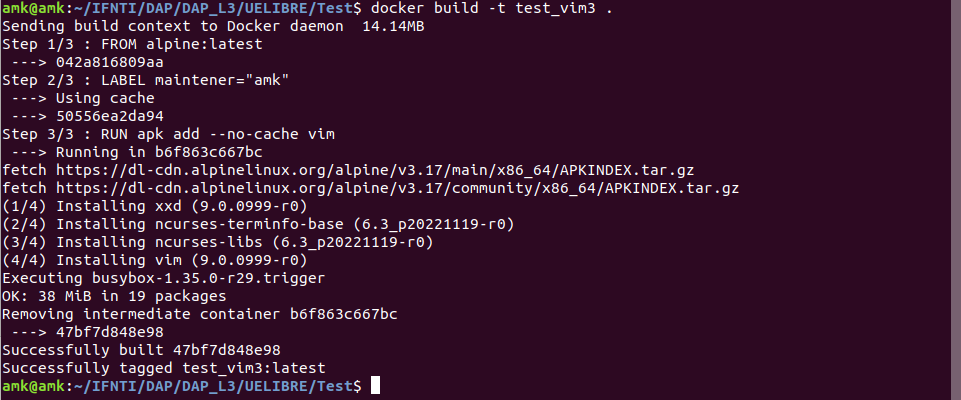
\includegraphics[scale=0.3]{img/test_vim_no_cache.png}
\end{center}
Donc on peut remarquer l'utilisation du cache au niveau de toute les couches sauf à la 
couche 3 c'est normale car nous n'avons spécifier l'utilisation du cache.
On peut aussi utiliser le --no-cache comme ceci :
\begin{verbatim}
docker build --no-cache -t test_vim2
\end{verbatim}
Mais là c'est l'intégralité du Dockerfile sur le quelle on n'appliquera pas de cache.

\textbf{NB } : l'ordre des éléments comptes. Il est important de mettre des instruction
caché en haut et ceux non caché tous en bas.
Exemple : Lancer successivement les Dockerfile suivant.\\
Dockerfile 1
\begin{verbatim}
FROM alpine:latest

LABEL maintener="amk"

ENV myvariable toto

RUN apk add  vim
\end{verbatim} 
\begin{verbatim}
docker build -t test
\end{verbatim}
\begin{verbatim}
docker build -t test1
\end{verbatim}
Dockerfile 2
\begin{verbatim}
FROM alpine:latest

LABEL maintener="amk"

ENV myvariable titi

RUN apk add  vim
\end{verbatim} 
\begin{verbatim}
docker build -t test
\end{verbatim}
Dockerfile 3
\begin{verbatim}
FROM alpine:latest

LABEL maintener="amk"

RUN apk add  vim

ENV myvariable toto
\end{verbatim} 
\begin{verbatim}
docker build -t test
\end{verbatim}

\section{Les Réseaux}
Le principale réseaux c'est le \textbf{Bridge} qu'on appelle le \textbf{Docker 0}.
Il à une adresse par défaut qui est le
\textbf{172.17.0.0/16}. Il permet la communication entre différent conteneurs et couvre 
la plus part des besoins en matière de réseau. Mais attention dans la manipulation des 
réseaux avec docker il est recommandé d'utiliser les nom des conteneur car les adresse 
ip ne sont pas fixe.

\subsection{ping sur le docker 0}
Avant de lancer un ping sur le docker 0 nous allons devoir d'abord créer un conteneur comme
ceci :
\begin{verbatim}
docker run -tid --name conteneur1 alpine
\end{verbatim}
Ensuit on rentre dans le conteneur en utilisant la commande suivante:
\begin{verbatim}
docker exec -ti conteneur1 sh 
\end{verbatim}
Une fois dans le conteneur on peut consulter son adresse ip avec la commande \textbf{ip a}.
\begin{center}
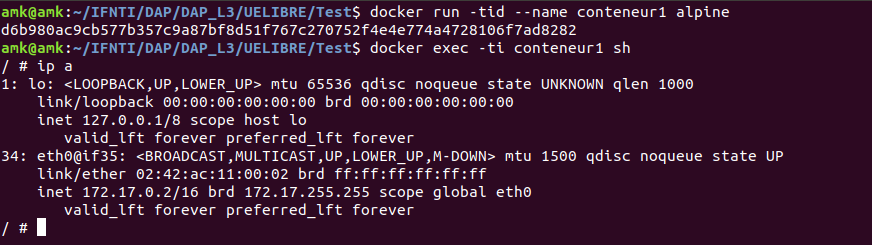
\includegraphics[scale=0.3]{img/ip_a_c1.png}
\end{center}
On peut remarqué que notre adresse ip commence à deux (2) au lieu de commencer à un (1).
Pourquoi ? car c'est le docker 0 qui est la première machine dans le \textbf{bridge}. On
peut lancer un ping vers ce docker 0 et ça marche car le conteneur est dans le même 
réseau que le docker 0.
\begin{center}
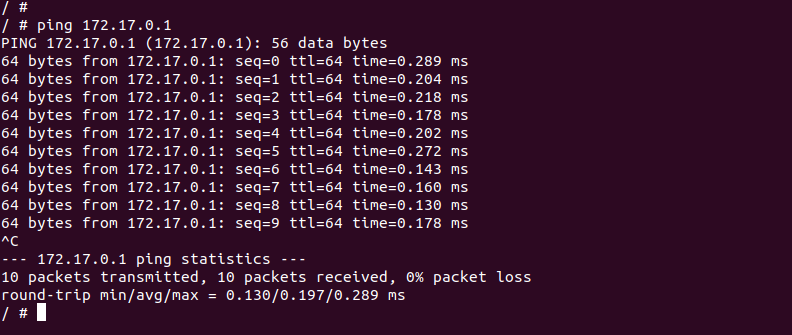
\includegraphics[scale=0.3]{img/ping_c1.png}
\end{center}

\subsection{Personnalisation du bridge --net}
Docker nous donne la possibilité de créer nos propres réseaux. Avant de créer notre premier 
réseau on va déjà regardé quelle sont les réseaux existant pour le moment. Pour le
faire lancé la commande :  \textbf{docker network ls} vous devriez avoir 
quelle que chose de similaire sans le \textbf{domalik\_default}.
\begin{center}
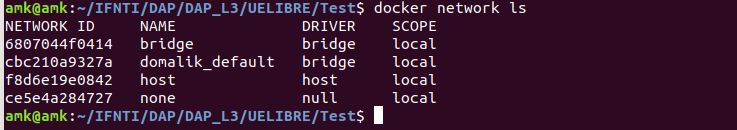
\includegraphics[scale=0.5]{img/d_networks.png}
\end{center}
Vous pouvez remarqué que les types de réseaux sont le \textbf{bridge}, le \textbf{host} et 
le \textbf{none}. Nous verrons ici comment créer des réseaux bridge.
Voici un exemple de réseau( de type bridge) dont le non est \textbf{mon\_reseau}et le sous
réseau est \textbf{172.30.0.0/16} on utilise
la commande
suivante :\\
\begin{verbatim}
docker network create -d bridge --subnet 172.30.0.0/16 mon_reseau
\end{verbatim}
Si vous fait un \textbf{docker network ls} vous verrez que le \textbf{mon\_reseau} à bien
été créé. En voici la preuve:
\begin{center}
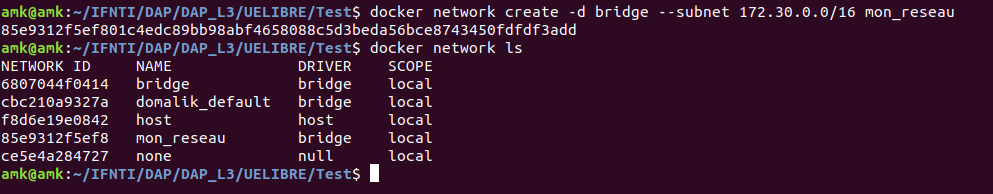
\includegraphics[scale=0.5]{img/my_network.png}
\end{center}
Pour faire un petit test de réseau on peut essayé de créer trois conteneur :
\begin{itemize}
\item deux première conteneur (conteneur1 et conteneur2) qui seront dans le même réseau et
\item un troisième conteneur qui sera dans le bridge par défaut.
\end{itemize}
Nous essayerons de lancer des ping de la manière suivante:
\begin{verbatim}
conteneur1   ------> conteneur2
conteneur2   ------> conteneur1
conteneur3   ------> conteneur1
\end{verbatim}
Sans plus tarder, créons les trois conteneurs :
\begin{verbatim}
docker run -itd --name conteneur1 --network mon_reseau alpine
docker run -itd --name conteneur2 --network mon_reseau alpine
docker run -itd --name conteneur3 alpine
\end{verbatim}
\begin{center}
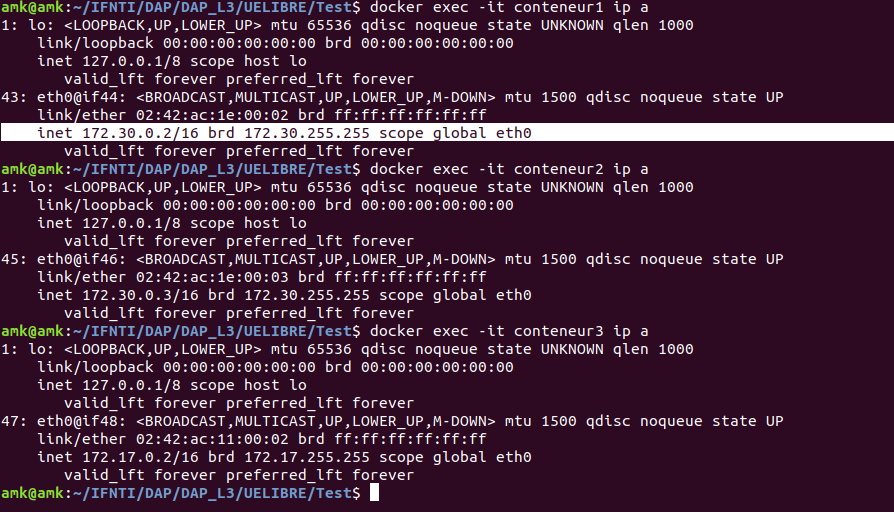
\includegraphics[scale=0.5]{img/ip_a_all_c.png}
\end{center}

\subsubsection{ping conteneur1 vs conteneur2}
\begin{center}
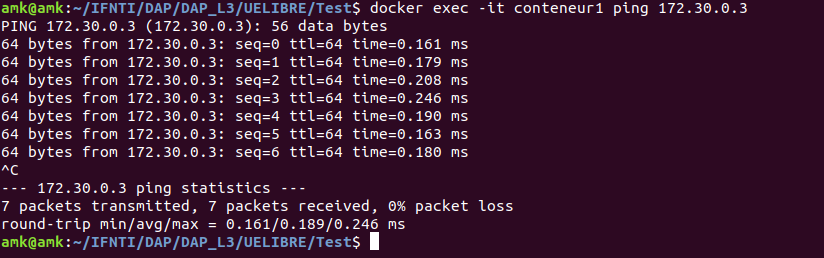
\includegraphics[scale=0.5]{img/ping_c1_c2.png}
\end{center}
Le ping marche car le conteneur1 et le conteneur2 sont dans le même sous réseaux.
\subsubsection{ping conteneur2 vs conteneur1}
\begin{center}
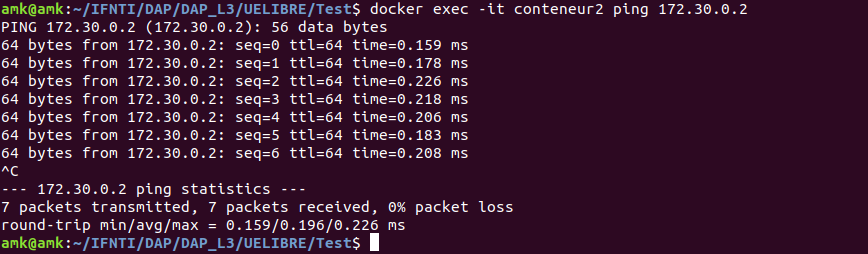
\includegraphics[scale=0.5]{img/ping_c2_c1.png}
\end{center}
Le ping marche car le conteneur1 et le conteneur2 sont dans le même sous réseaux.
\subsubsection{ping conteneur3 vs conteneur1}
\begin{center}
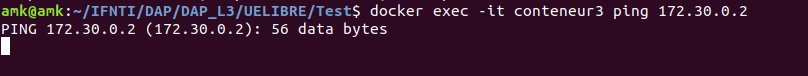
\includegraphics[scale=0.5]{img/ping_c3_c1.png}
\end{center}
Le ping ne marche pas car le conteneur1 et le conteneur3 ne sont pas dans le même sous
 réseaux.
 
\subsection{Autre cas --net}
\begin{itemize}
\item \textbf{--net : none} Pour spécifier que le conteneur n'a aucune ouverture réseau 
(cas particulier).
\item \textbf{--net : host} Son ouverture réseau ne correspond qu'a l'accès au host.
\item \textbf{--net : container:<nomconteneur>} Ouverture réseau à un conteneur particulier.
\end{itemize}

\subsection{Autre cas --link}
\textbf{--link : container:<nomconteneur>} Ouverture réseau à un conteneur particulier. Mais vas aller compléter le \textbf{/etc/hosts} du conteneur.\\
Pour tester ça : on vas créer deux conteneurs. Le conteneur1 et le conteneur2 qui
utilise le réseau du conteneur2
\begin{verbatim}
docker run -itd --name conteneur1 alpine
docker run -itd --name conteneur2 --link conteneur1 alpine
\end{verbatim}
\begin{center}
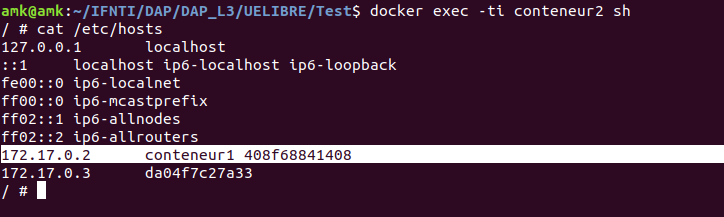
\includegraphics[scale=0.5]{img/link_c1.png}
\end{center}

\subsection{Et en plus ...}
\begin{itemize}
\item \textbf{--add-host <nomhost>:ip} : complète le /etc/hosts.
\item \textbf{--dns} : ajoute les ip de serveurs dns.
\end{itemize}

Test : ici nous avons créer le conteneur1 en précisant l'option --add-host pour cela 
demander à un de vos camarade de vous donner son adresse ip ou si vous aviez une deuxième
machine prenez son adresse ip. Dans mon cas l'adresse ip de mon camarade est le 
\textit{192.168.60.180}(Il est important que votre host soit aussi dans le sous réseau). 
\begin{center}
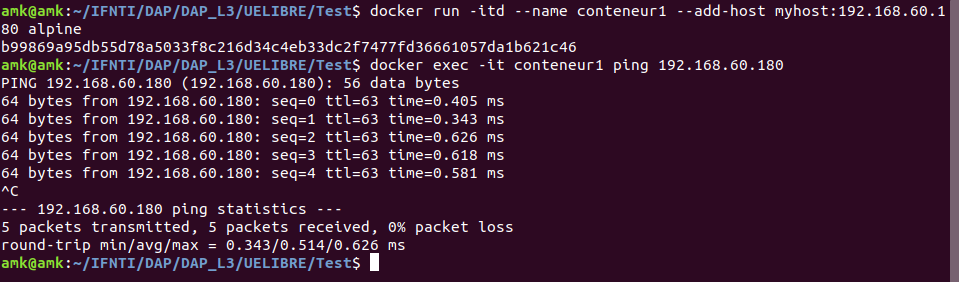
\includegraphics[scale=0.5]{img/add_host.png}
\end{center}
\begin{center}
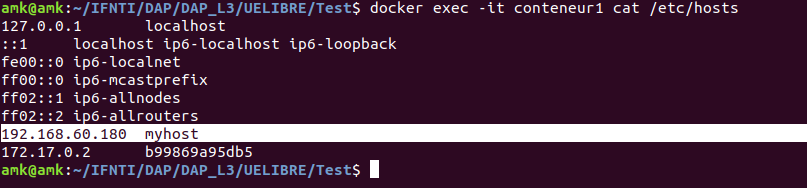
\includegraphics[scale=0.5]{img/add_host_2.png}
\end{center}

\section{Docker compose}


\end{document}



